\documentclass{article}
\usepackage{amsfonts}
\usepackage{textcomp}
\usepackage{amsmath}
\usepackage{graphicx}
\begin{document}

\pagebreak	
\section{Technical Description}
\subsection{Notational Note}
When denoting vector or matrix variables I use a capital letter to indicate the entire structure and an indexed lowercase letter to indicate a specific component value.
As illustration 
$X=  \begin{bmatrix}
x^{(0)}_{11}  & \dots & x^{(0)}_{1n}& \dots& x^{(0)}_{1N} \\
\hdotsfor{5} \\
x^{(0)}_{m1}        & \dots& x^{(0)}_{mn} & \dots& x^{(0)}_{mN}\\
\hdotsfor{5}\\
x^{(0)}_{M1}        & \dots & x^{(0)}_{Mn}& \dots &x^{(0)}_{MN}
\end{bmatrix}$

When denoting indices I use a Mathcal formatted letter to represent the set of indices, the lowercase letter to indicate an element from the set of indices and the capital letter to indicate the largest value in the set of indices.    As Illustrstion\\
$\mathcal{J}=\{1,...j,...J\}$

\subsection{The Network Architecture}
Experiments part 2 and part 3 both take the form of a neural network with the generic architecture of an input layer, a convolutional network with a specified quantity of convolutional filters, a flattening of the convolutional network outputs, a multilayer perceptron and then an output.   TODO show picture here.  Although these two parts are listed as seperate for the project description it is easiest to view them as the same structure of network with different hyperparameters.  Consequently in the mathematical derivations and code implementation I describe the network generically using variables for all hyperparameters distinguishing these two project components.  In the experimetn section I describe the specific values taken on by certain variables.

\subsection{The Math of training our Network}
\subsubsection{forward}
I first mathematically characterize our traing data set as the following

\begin{equation}\label{eq:1}
D = \{X^{(0)}(t), P(t)\},
X^{(0)}=  \begin{bmatrix}
x^{(0)}_{11}  & \dots & x^{(0)}_{1c}& \dots& x^{(0)}_{1D} \\
\hdotsfor{5} \\
x^{(0)}_{c1}        & \dots& x^{(0)}_{cd} & \dots& x^{(0)}_{cD}\\
\hdotsfor{5}\\
x^{(0)}_{C1}        & \dots & x^{(0)}_{Cd}& \dots &x^{(0)}_{CD}
\end{bmatrix},P(t) \in \mathbb{Z}_{R} 
\end{equation}

Here $t$ is used to denote the index of our training sample in the dataset. The variable $X(t)^{(0)}$ refers to the $t$th sample of our data set and $P(t)$ refers to the corresponding label for that training sample. Our $P(t) \in \mathbb{R}$, where $R$ is the number of possible labels and the space $\mathbb{R}$ is one-hot encoded so that it can be expressed by the output layer of our perceptron as well as for other computational purposes that are outlined in \ref{}. Each training sample is a matrix of dimension $C$x$D$. 

The first hidden layer applied to the input sample of our network is the convolutional layer.  The convolutional layer is defined by a kernel 
\begin{equation}
A^{(0)}_l=  \begin{bmatrix}
a^{(0)}_{11}  & \dots & a^{(0)}_{1n}& \dots& a^{(0)}_{1J} \\
\hdotsfor{5} \\
a^{(0)}_{i1}        & \dots& a^{(0)}_{ij} & \dots& a^{(0)}_{iJ}\\
\hdotsfor{5}\\
a^{(0)}_{I1}        & \dots & a^{(0)}_{Ij}& \dots &a^{(0)}_{IJ}
\end{bmatrix}
\end{equation}. I combine all filters into one tensor $A$ where $l$ denotes the index of the filter and $m$ and $n$ are the indices of the receptive field. I know through convolutional arithmetic that 
\begin{equation}
M=C-I+1,
N=D-J+1.
\end{equation} This is, ofcourse, assuming that the stride is $1$ and that the convolution operation conatins no padding.
 Each filter $A^({0})_l$ will be convoled across the input layer show in the following equation.
\begin{equation}
	Z^{(0)}_{l,m,n} = \sum_{j\in \mathcal{J}}\sum_{i \in \mathcal{I}}a_{l,i,j} x^{(0)}_{m+i, n+j}+b^{(0)}_{l}
\end{equation}.  In this case $b_l$ denotes the bias of filter $l$. It is worth noting that in this notation the convolutional layer is subject to the constraint that all filters in at a given convolutional layer are the same size, which is not always the case, but is satisfied in all stages of this project.

After the inputs have passed through the convolution layer I apply a non-linear activation function
\begin{equation}
	X^{(1)}_{l,m,n} = \sigma^{(1)}(Z_{l,m,n})
\end{equation}
I denote the generic non-linear activation as $\sigma$ and describe the different non-linearities considered in the section \ref{Non-Linearities}

After our training data has passed through the non-linearity it must traverse through the perceptron Layer.  However, because of the current formulation of our convolutional layer our data is a tensor of shape (L,M-I, N-J). A fully conencted perceptron expects a 1-dimensional input so it is necessary to flatten the tensor out.  This simply involves unrolling along the dimensions of our tensor via the equation
\begin{equation}
V^{(1)} =  flatten(X^{(1)}_{l,m,n}) = 
\begin{bmatrix}
v^{(1)}_{1} & \dots &v^{(1)}_{k} 
\end{bmatrix}
\end{equation} and re-indexing the flattened layer with the variable 
\begin{equation}
k = l*NM+m*N+n.
\end{equation}  We note that $K=L*(M-I)*(N-J)$.
Now that we have a 1-dimensional input we pass it to the perceptron layer defined by the weights and bias.
\begin{equation}
W^{(0)}=  \begin{bmatrix}
w^{(0)}_{11}  & \dots & w^{(0)}_{1k}& \dots& w^{(0)}_{1K} \\
\hdotsfor{5} \\
w^{(0)}_{r1}        & \dots& w^{(0)}_{rk} & \dots& w^{(0)}_{rK}\\
\hdotsfor{5}\\
w^{(0)}_{R1}        & \dots & w^{(0)}_{Rk}& \dots &w^{(0)}_{RK}
\end{bmatrix},
b^{(1)}
\end{equation}
Where $R$ is the desired number of outputs.  Note that this $R$ is the same $R$ as is seen in equation \ref{eq:1}, because the output of our perceptron will be compared against the label of the datapoint we are currently observing.  We pass the data through this layer via the qeuation
\begin{equation}
z^{(1)}_{r} = \sum_{k\in\mathcal{K}}w_{r,k}v_{k}+b^{(1)}	
\end{equation}.  

We then apply a second non-linear activation function.
\begin{equation}
x^{(2)}_{1} = \sigma^{(2)}(z^{(1)}_r).
\end{equation}
The output of this non-linear activation will now be treated as a prediction for the label $P(t)$.  We evaluate the effectiveness of this forward pass in predicting the label by using the vector $X^{(2)}$ and $P(t)$ as inputs to an error function which I denote generically as
\begin{equation}
E(X^{(2)}(t), P(t)).
\end{equation}  We describe the different erorr functions considered in \ref{error}


\subsection{BackPropagation}
My network is structured so that there are 4 different classes of parameters to tune.  The weights and bias of the perceptron and the weights and bias of the convolutional kernels.  We denote them with the following partials:
\begin{equation}
\frac{\partial E}{\partial w_{r,k}},
\frac{\partial E}{\partial b^{(1)}},
\frac{\partial E}{\partial a_{l,i,j}},
\frac{\partial E}{\partial b^{(0)}_{l}}
\end{equation} 
and evaluate them via the chain rule
\begin{equation}
\frac{\partial E}{\partial w_{r,k}} =
\frac{\partial E}{\partial x_{r}^{(2)}}
\frac{\partial x^{(2)}_{r}}{\partial z_{r}^{(1)}}
\frac{\partial z_{r}^{(1)}}{\partial w_{r,k}}
\end{equation}

\begin{equation}
\frac{\partial E}{\partial b^{(1)}} =
\frac{\partial E}{\partial x_{r}^{(2)}}
\frac{\partial x^{(2)}_{r}}{\partial z_{r}^{(1)}}
\end{equation}

\begin{equation}
\frac{\partial E}{\partial a_{l,i,j}} = 
\sum_{r\in \mathcal{R}}
\frac{\partial E}{\partial x_{r}^{(2)}}
\frac{\partial x_{r}^{(2)}}{\partial z_{r}^{(1)}}
\sum_{n\in \mathcal{N}}
\sum_{m\in \mathcal{M}}
\frac{\partial z_{r}}{\partial x^{(1)}_{l,m,n}}
\frac{\partial x^{(1)}_{l,m,n}}{\partial z^{(0)}_{l,m,n}}
\frac{\partial z_{l,m,n}^{(0)}}{ \partial a_{l,i,j}}
\end{equation}

\begin{equation}
\frac{\partial E}{\partial b_{l}} = 
\sum_{r\in \mathcal{R}}
\frac{\partial E}{\partial x_{r}^{(2)}}
\frac{\partial x_{r}^{(2)}}{\partial z_{r}^{(1)}}
\sum_{n\in \mathcal{N}}
\sum_{m\in \mathcal{M}}
\frac{\partial z_{r}}{\partial x^{(1)}_{l,m,n}}
\frac{\partial x^{(1)}_{l,m,n}}{\partial z^{(0)}_{l,m,n}}
\end{equation}

After these partials are determined we can use them to update the weights and biases of the convolutional kernels and perceptrion. 

\begin{equation}
w_{r,k} := w_{r,k}- \alpha * \frac{\partial E}{\partial w_{r,k}}
\end{equation}
\begin{equation}
b^{(1)} := b^{(1)} - \alpha* \frac{\partial E}{\partial b^{(1)}}
\end{equation}
\begin{equation}
a_{l,i,j} := a_{l,i,j} - \alpha*\frac{\partial E}{\partial a_{l,i,j}}
\end{equation}
\begin{equation}
b^{(0)} := b^{()_{l}} - \alpha*\frac{\partial E}{\partial b^{(0)}_{l}}
\end{equation}
Here, $\alpha$ represents the learning rate of our network.

The next subsections discuss a few of the posisble values for the component partials which make up these equations

\subsubsection{Error Functions}\label{error}
Most of our experiments are run using the squared error function
\begin{equation}
E_{squared-error}(X^{(2)}(t), P(t)) =  \frac{1}{2}\sum_{r\in\mathcal{R}}(x^{(2)}_{r}(t)-P(t))^2.
\end{equation}
Taking the partial as will be used for backpropagation we see
\begin{equation}
\frac{\partial E}{\partial x_r^{(2)}}= x^{(2)}_{r}-P(t)
\end{equation}

\subsection{Activation Functions}\label{activation}
We consider multiple different activation functions.
The first activation function considered is the hyperbolic tangent denoted
\begin{equation}
x = \sigma_{th}(z) = \frac{e^{(2z)}-1}{e^{(2z)}+1}
\end{equation}.
The tangent
\begin{equation}
\frac{\partial \sigma_{th}}{\partial z} = 1 - \sigma_{t}(z)
\end{equation}
\begin{equation}
x = \sigma_{s}(z) = \frac{1}{1+e^{-z}}
\end{equation}
\begin{equation}
\frac{\partial \sigma_{s}}{\partial z} = \sigma_{s}(z)(1-\sigma_{s}(z))
\end{equation}
Both of these activation functions have an advantage of their partials being functions of the activation function.  This is useful in computation of gradients during backpropagation 

\pagebreak
\section{Code Description}
The files used in this report are stored the directory tree shown below.

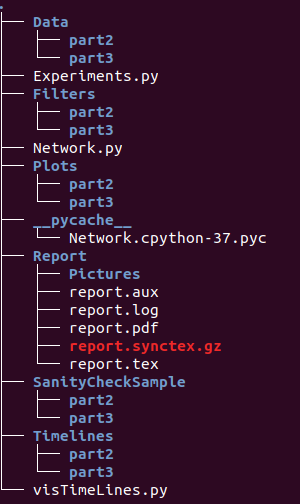
\includegraphics[scale=.5]{Pictures/Tree.png}
\includegraphics[scale=.5]{Pictures/freez0}

The python module {\it Network.py} is where the Network is defined. Module contains the following Methods:\\
\# Loss Functions:\\
SquaredError\\
\# Activation Functions:\\
 tanhAct, sigmoidAct, reluACt, noAct\\
\# Auxillary Functions:\\
 SaveImagesAndTimelines
 getTrainingData, DecisionLayer\\
\# runNetwork 

The bulk of the computations are performed in the {\it runNetwork} method.   The method takes one dictionary parameter which contains all configuration settings that define an individual experiment including auxilarry information and hyperparameters. With the variables I tried to make the notation as consistent as possible with the derivations outlined in the paper. 

The {\it runNetwork()} method is called with various iterations of the potential parameters within the {\it Experiments.py} module. 
The possible configurations settings are as follows:

\begin{table}[]
\begin{tabular}{l|llll}
 Epochs& number of Epochs    &  &  &  \\
 ExNum & Part Num            & 2,3&  &  \\
 T     & Num Train Sample    & 32,100 &  &  \\
 TT    & Num Test  Sample    & 98,100 &  & \\
 L     & num Conv Layers    & Int & \\
 I     & conv Kernel Height  & Int &  & \\
 J     & conv Kernel Width   & Int &  & \\
 C     & Image Height        & Int &  & \\
 D     & Image Width         & Int &  & \\
 R     & Perceptron Outputs  & 2,20 &  & \\
 lrW   & Learning Rate       & Float &  & \\
 lrA   & Learning Rate Conv  & Float &  & \\
 ACT   & Activation Function & tanhAct, sigmoidAct, reluAct, noAct &  & \\
 LOSS  & Loss Function       & SquaredError  &  & \\
ORDER& Order of training Data&Fixed, Shuffle, Random\\
 vis   & Visualize Data      & True,False &  & \\
\end{tabular}
\end{table}


\section{Experiments}
\subsection{Order}
I run the network for experiment 2 in three different orders: Fixed, Shuffled, and Random.  With the sequential ordering I train over all samples with label $1$ followed by all samples with label $3$.  In Shuffled I mix the training data so that it alternates between samples of $3$ and $1$ every iteration.  With random I present the samples to the network in a random ordering.  In all three orderings the Network is presented each sample once per epic

	
\subsection{Learning Rate}
I run the network with across learning rates increasing by powers of 10.
$\alpha \in \{0.1, 0.01, 0.001, 0.0001\}$

\subsubsection{Varied Learning Rates}
In noticed that when looking at the partials $\frac{\partial E}{\partial W}$ and $\frac{\partial E}{\partial K}$ that the partials were significiantly larger in $\frac{\partial E}{\partial W}$.  In retrospect this makes sense as the convolutional layer occurs later in the backpropogation step.  I know that this phenomenon is referred to the vanishing gradient problem and often occur in deeper networks, but did not realize it would happen in a network as shallow as this one.  I adjusted the network so that rather than applying a universal learning rate to all gradient descent steps I used a larger learning rate for the convolutional kernels.
$\alpha_a = 0.01$ $\alpha_w = 0.0001$

\subsection{Freezing Perceptron Weights}

\includegraphics[scale=.5]{Pictures/freez0}

\subsection{Debuging error}
I am fairly certain there is a single, minor error somewhere in my code that is negatively impacting the results of these experiments.  Because of the way this was coded up the parameters for number of filters and filter size do not alter implementation and the only thing differentiating part 3 and part 2 is some configuration settings.  



\end{document}